\chapter{Comparison in the Time and Frequency Domains}

This chapter aims to validate the implementation of the two instrumental noise models introduced in Chapter~4. In particular, the objective is to verify that the statistical properties of the generated Time-Ordered Data are consistent in both the time domain and the frequency domain.

To this end, both noise-generation methods are tested under identical simulation conditions. The same detector parameters, scanning strategy, observation duration, and random seeds are used for the two models. The resulting TODs are then analyzed and compared through time-domain plots and power spectral density (PSD) estimates.



\section{Short-Time Simulations Setup}

Time-domain and frequency-domain analyses are based on a consistent simulation setup applied to both noise-generation methods.

The total observation time is chosen on the order of $10^3$ seconds, sufficient to reveal the characteristic $1/f$ behavior while keeping simulations computationally lightweight. Two detector types are considered: a custom detector and an IMo-based detector. Due to the lower knee frequency of the IMo detector ($f_\text{knee} = 20$~mHz vs.\ $500$~mHz for the custom detector), IMo simulations are extended to $8000$~s, compared to $1000$~s for the custom detector, ensuring that slow temporal drifts and the transition to the white-noise plateau are observable. For each detector, the simulation duration is identical across the \texttt{add\_lbsNoise} and \texttt{add\_OofaNoise} runs, so that any differences originate solely from the noise-generation method.

A simple scanning strategy is implemented: the satellite rotates around a fixed spin axis aligned with the Earth--Sun direction at $1/60$~Hz (one rotation per minute), and the telescope line of sight forms a $90^\circ$ angle with the spin axis. 

The scanning strategy is sampled at a time interval of 5 s, corresponding to the frequency at which the LBS framework recalculates the spacecraft's orientation. The attitude is represented using quaternions, and the pointings required at the detector sampling frequency (20 Hz for the custom detector and 31 Hz for the IMo detector) are obtained via spherical linear interpolation of the quaternions (SLERP). In this way, the attitude recalculation interval can be longer than the detector sampling period (the recalculation frequency can be lower than the sampling frequency) because the pointings at intermediate times are accurately reconstructed through quaternion interpolation.


Detector parameters, including sampling frequency, NET, knee frequency, minimum frequency, spectral index $\alpha$, and band center, are kept identical between the two noise models. Table~5.1 summarizes the values used.

\begin{table}[h]
\centering
\begin{tabular}{lcc}
\hline
\textbf{Parameter} & \textbf{Custom Detector} & \textbf{IMo Detector} \\
\hline
Sampling rate [Hz] & $20.0$ & $31.0$ \\
Band center [GHz] & $100.0$ & $40.0$ \\
NET [$\mu$K$\sqrt{\mathrm{s}}$] & $50.0$ & $114.63$ \\
Knee frequency [mHz] & $500.0$ & $20.0$ \\
Minimum frequency [Hz] & $1\times10^{-5}$ & $1\times10^{-5}$ \\
Spectral index $\alpha$ & $1.0$ & $1.0$ \\
\hline
\end{tabular}
\caption{Detector parameters used in the short-time simulations for the custom and IMo detectors.}
\end{table}

To ensure reproducibility, the random number generator is initialized with a fixed seed, identical across both noise-generation methods. The observation data structure is then created, and instrumental noise is added to the TOD using either \texttt{add\_lbsNoise} or \texttt{add\_OofaNoise}. The temporal block for noise generation is set to $100$~s, long enough to capture the $1/f$ correlations ($\tau_\text{knee} \sim 1/f_\text{knee}$) but short relative to the total simulation duration. 

The simulated TOD contains only instrumental noise and is expressed in units of equivalent CMB temperature ($\mu$K$_\mathrm{CMB}$), allowing direct comparison with theoretical maps and instrumental sensitivity estimates. Any differences observed in time or frequency domain analyses therefore arise exclusively from the chosen noise-generation strategy.




\section{Time-Domain Analysis}

After adding instrumental noise to the TOD, time-domain plots display the noise amplitude ($\mu$K) as a function of time (s), allowing direct visual inspection of temporal correlations.

$1/f$ noise manifests as slow, coherent variations over time, in contrast to white noise, which fluctuates rapidly and independently around zero. These low-frequency drifts introduce memory into the signal, producing gradual waves lasting hundreds of seconds. Visual inspection of the TOD therefore provides a clear qualitative signature of the $1/f$ component.

Figures~5.1 and 5.2 show TODs generated with the custom detector. 

The fluctuation amplitude remains within $\pm 500~\mu\mathrm{K}$, consistent with the NET value of $50~\mu\mathrm{K}\sqrt{\mathrm{s}}$. For white noise, the per-sample standard deviation is
\[
\sigma_{\mathrm{white}} = \mathrm{NET} \cdot \sqrt{f_{\mathrm{samp}}} \simeq 223.6~\mu\mathrm{K},
\]
which agrees with the observed range. Looking at the plots, most samples indeed fall within approximately $\pm 500~\mu\mathrm{K}$, corresponding to roughly $2$–$3\,\sigma$. In a Gaussian distribution, 99.7\% of the data lies within $\pm 3\,\sigma$ of the mean, so a visual range of about $\pm 700~\mu\mathrm{K}$ is fully consistent with the theoretical expectations.

In block-based FFT generation (\texttt{add\_lbsNoise}), one might expect discontinuities at the block boundaries, since each segment is generated independently. In practice, these jumps are negligible: high-frequency white noise fluctuations are much larger than any systematic jump from phase truncation, and with $\alpha=1$ the energy in very low frequencies is spread over long timescales, making block-to-block deviations comparable to normal signal fluctuations.

Both noise-generation methods produce statistically consistent TODs:
\begin{itemize}
    \item \texttt{add\_lbsNoise} exhibits slightly more jagged fluctuations due to the FFT-based block generation;
    \item \texttt{add\_OofaNoise} yields smoother low-frequency variations, reflecting the effectiveness of the continuous filtering.
\end{itemize}

\begin{figure}[h!]
    \centering
    
\includegraphics[width=0.68\textwidth]{tod_mock_lbs.pdf}
    \caption{TOD simulated with the custom detector using \texttt{add\_lbsNoise}.}
    \label{fig:tod_custom_lbs}
\end{figure}

\begin{figure}[h!]
    \centering
    
\includegraphics[width=0.68\textwidth]{tod_mock_oofa.pdf}
    \caption{TOD simulated with the custom detector using \texttt{add\_OofaNoise}.}
    \label{fig:tod_custom_oofa}
\end{figure}

The analysis was repeated using a real IMo detector (\texttt{000\_000\_008\_UA\_040\_T}) with a low knee frequency ($f_\mathrm{knee}=20$~mHz) and extended duration ($8000$~s). The theoretical white-noise standard deviation is $\sigma_\mathrm{white} \simeq 638~\mu$K, and the TOD shows fluctuations up to $\pm 2000~\mu$K, consistent with Gaussian statistics.

Due to the low $f_\mathrm{knee}$, slow drifts appear less frequent than in the custom detector, as white noise dominates over a broader frequency range. Nevertheless, both \texttt{add\_lbsNoise} and \texttt{add\_OofaNoise} correctly scale the noise amplitude according to NET and sampling frequency, with \texttt{add\_OofaNoise} producing smoother transitions between fast and slow fluctuations.


\begin{figure}[h!]
    \centering
    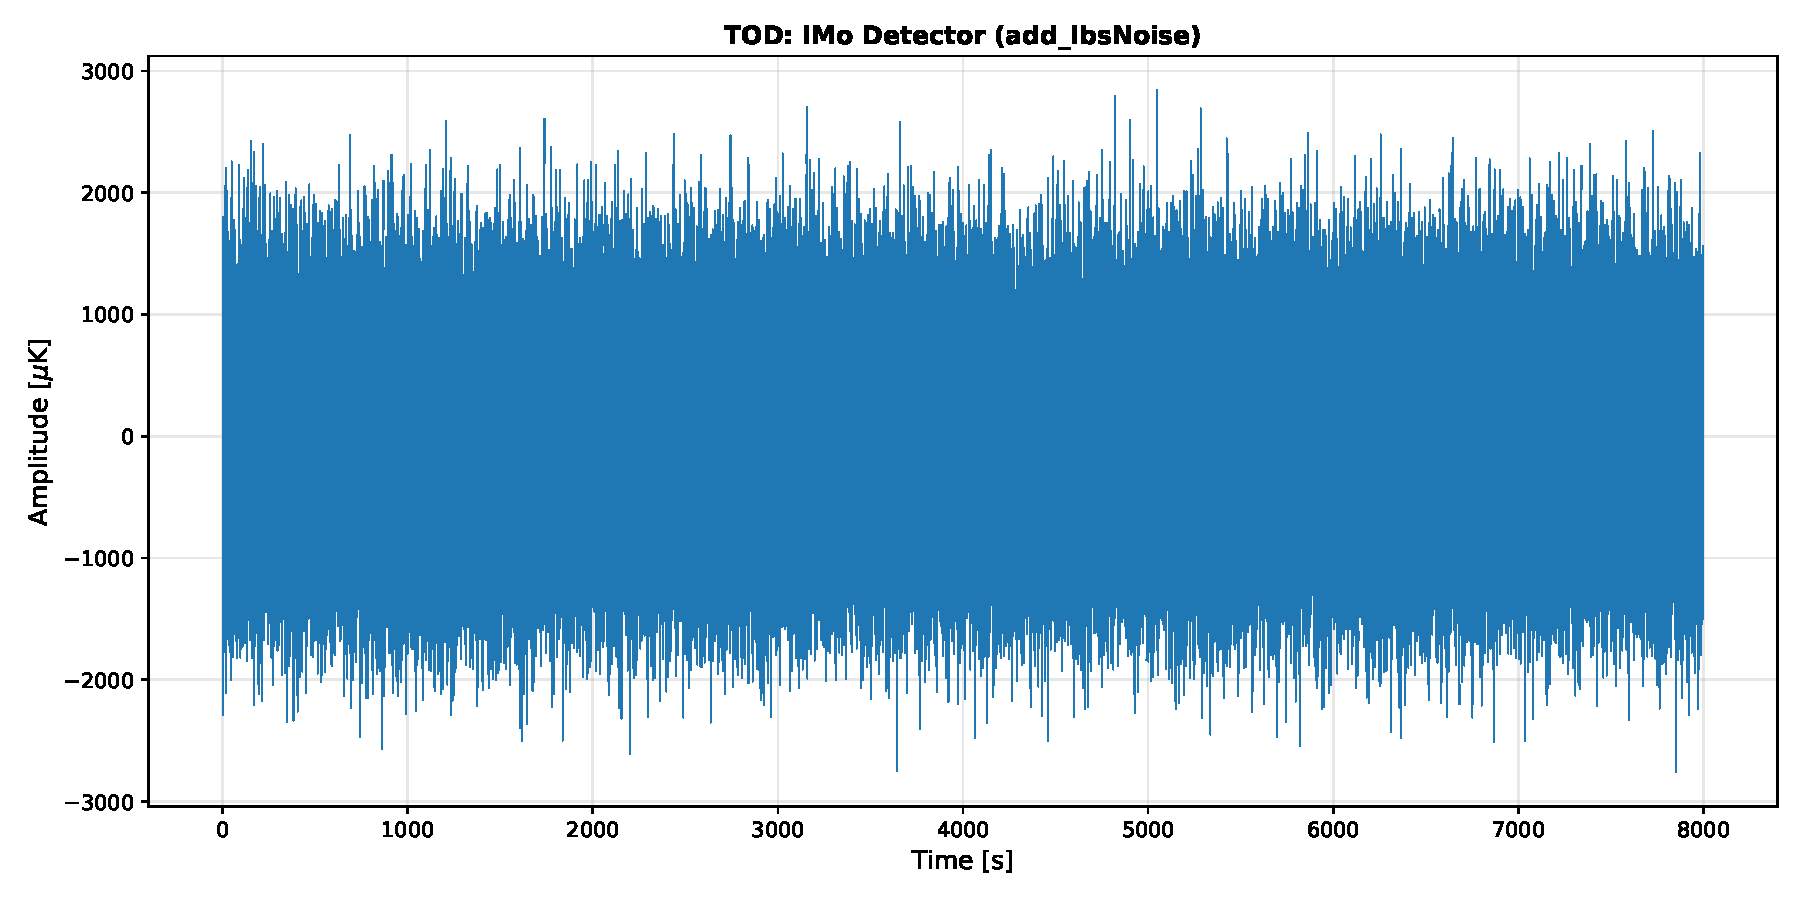
\includegraphics[width=0.68\textwidth]{tod_imo_lbs.pdf}
    \caption{TOD simulated with the IMo detector using \texttt{add\_lbsNoise}.}
    \label{fig:tod_imo_lbs}
\end{figure}

\begin{figure}[h!]
    \centering
    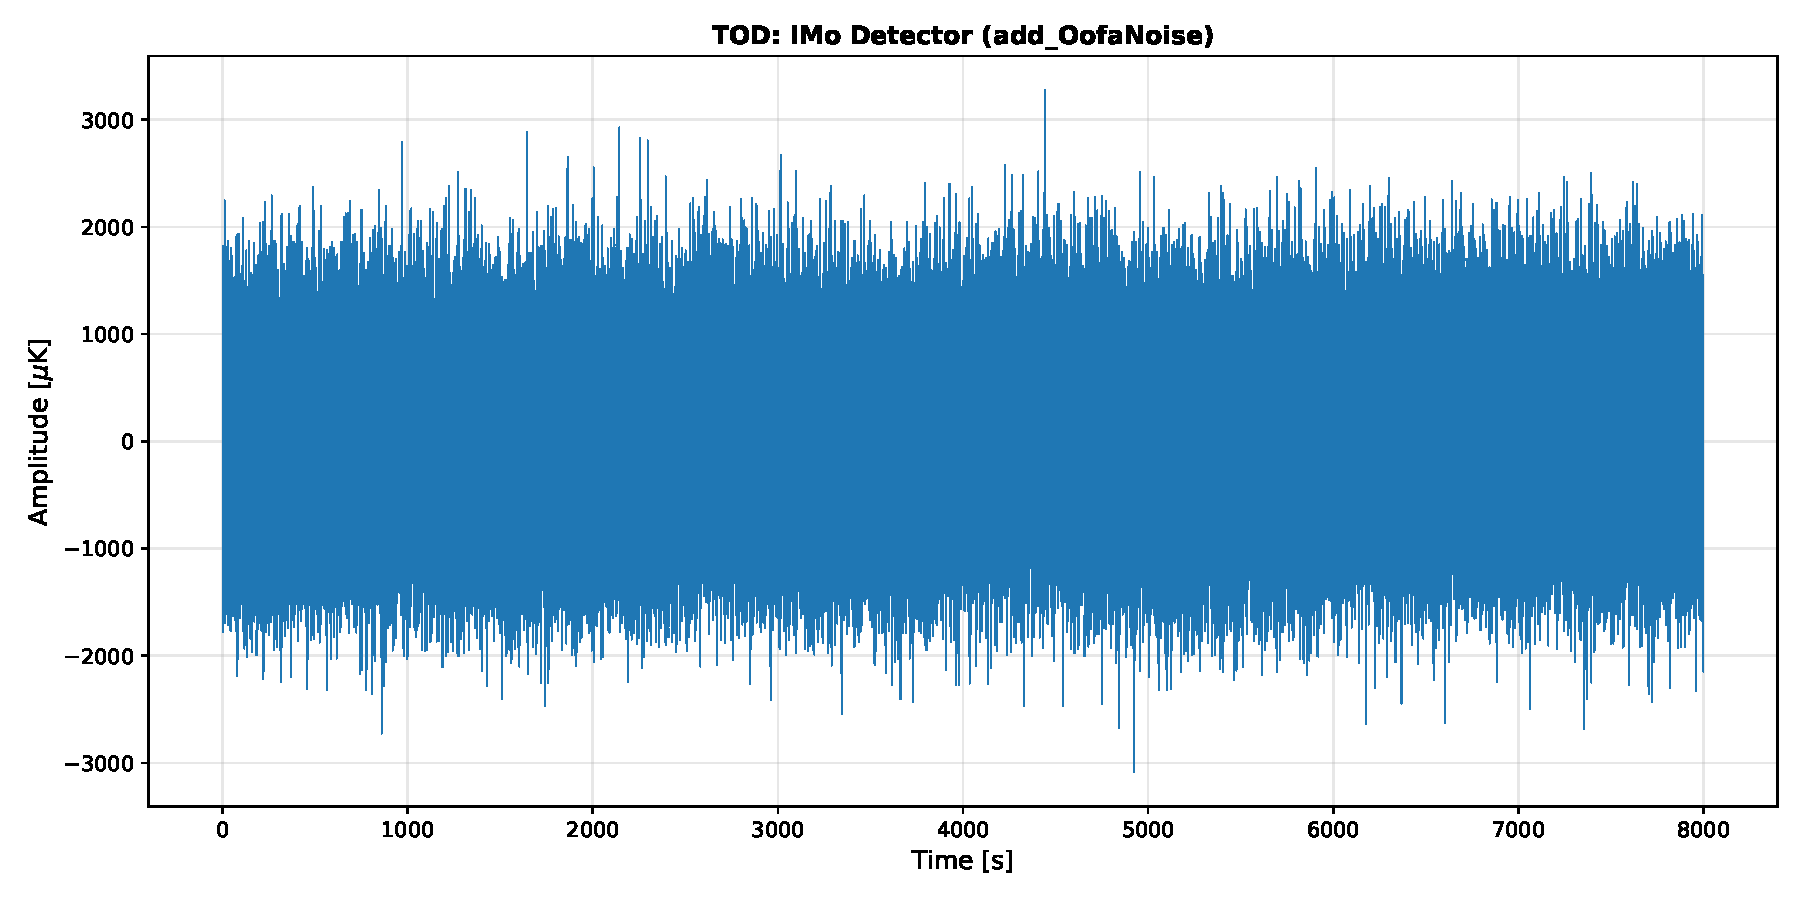
\includegraphics[width=0.68\textwidth]{tod_imo_oofa.pdf}
    \caption{TOD simulated with the IMo detector using \texttt{add\_OofaNoise}.}
    \label{fig:tod_imo_oofa}
\end{figure}

In summary, the time-domain analysis confirms that both models reproduce the expected statistical power and phenomenology of $1/f$ noise, independently of detector choice. The custom detector highlights the $1/f$ behavior over short timescales, while the IMo detector illustrates the dominance of white noise in realistic mission conditions, justifying the need for frequency-domain analysis.




\section{Frequency-Domain Analysis}

After validating the noise models in the time domain, their statistical properties are verified in the frequency domain by comparing the PSD of the simulated TODs with the theoretical model from Chapter~2:

\begin{equation} 
P(f) = \mathrm{NET}^2 \left[ \frac{f^\alpha + f_{knee}^\alpha}{f^\alpha + f_\text{min}^\alpha} \right]. 
\end{equation}  

Spectral analysis clearly separates the white-noise contribution (high frequencies) from the $1/f$ component (low frequencies) and allows verification of the knee frequency $f_\mathrm{knee}$ and spectral index $\alpha$.

The Welch method is adopted to estimate the PSD, reducing variance compared to a simple periodogram. Signals are divided into overlapping segments, windowed with a Hann function, and averaged to obtain a stable spectrum.

For both noise-generation methods and detector types, the Welch parameters are:
\begin{itemize}
    \item Segment length $\text{nperseg}=2^{12}$ samples, yielding a frequency resolution $\Delta f = \frac{\text{nperseg}}{f_{\mathrm{samp}}} \simeq 5$--$7$~mHz for $f_\mathrm{samp}=20$--$31$~Hz, sufficient to resolve the knee and the $1/f$ slope.
    \item $50\%$ overlap to improve averaging without significant computational cost.
    \item Hann window to minimize spectral leakage (the spreading of energy from one frequency to other frequencies) at segment boundaries.
    \item Density scaling in $\mu\mathrm{K}^2/\mathrm{Hz}$.
\end{itemize}

Figures 5.5 and 5.6 show the PSD for the custom detector ($f_{\text{knee}} = 0.5$~Hz, $\mathrm{NET} = 50~\mu\text{K}\sqrt{\text{s}}$). At high frequencies ($f > 1$~Hz), both methods converge to the expected white-noise plateau at $\mathrm{NET}^2 = 2500~\mu\text{K}^2/\text{Hz}$. Below the knee frequency, the spectrum follows the $f^{-\alpha}$ behavior, confirming the presence of the correct long-term correlations. The transition between the white-noise regime and the correlated-noise regime occurs at the expected knee frequency, $f_\mathrm{knee} = 0.5$~Hz.

No significant differences between \texttt{add\_lbsNoise} and \texttt{add\_OofaNoise} are observed. These PSDs are computed directly from the TODs analyzed in Section~5.2, ensuring consistency with time-domain observations.

\begin{figure}[h!]
    \centering
    
\includegraphics[width=0.68\textwidth]{psd_mock_lbs.pdf}
    \caption{PSD of the TOD simulated with the custom detector using \texttt{add\_lbsNoise}.}
    \label{fig:psd_custom_lbs}
\end{figure}

\begin{figure}[h!]
    \centering
    
\includegraphics[width=0.68\textwidth]{psd_mock_oofa.pdf}
    \caption{PSD of the TOD simulated with the custom detector using \texttt{add\_OofaNoise}.}
    \label{fig:psd_custom_oofa}
\end{figure}



The analysis was repeated for the IMO detector ($f_{\text{knee}} = 20$~mHz, $\mathrm{NET} = 114.63~\mu\text{K}\sqrt{\text{s}}$). The resulting PSDs highlight a high-frequency plateau stabilizing around $\mathrm{NET}^2 \simeq 1.3 \times 10^4~\mu\text{K}^2/\text{Hz}$. Despite the relatively low knee frequency being close to the spectral resolution limit of the analysis (approximately $7$~mHz), the characteristic $1/f$ rise remains clearly visible in the spectrum, emerging around $0.02$~Hz.

\begin{figure}[h!]
    \centering
    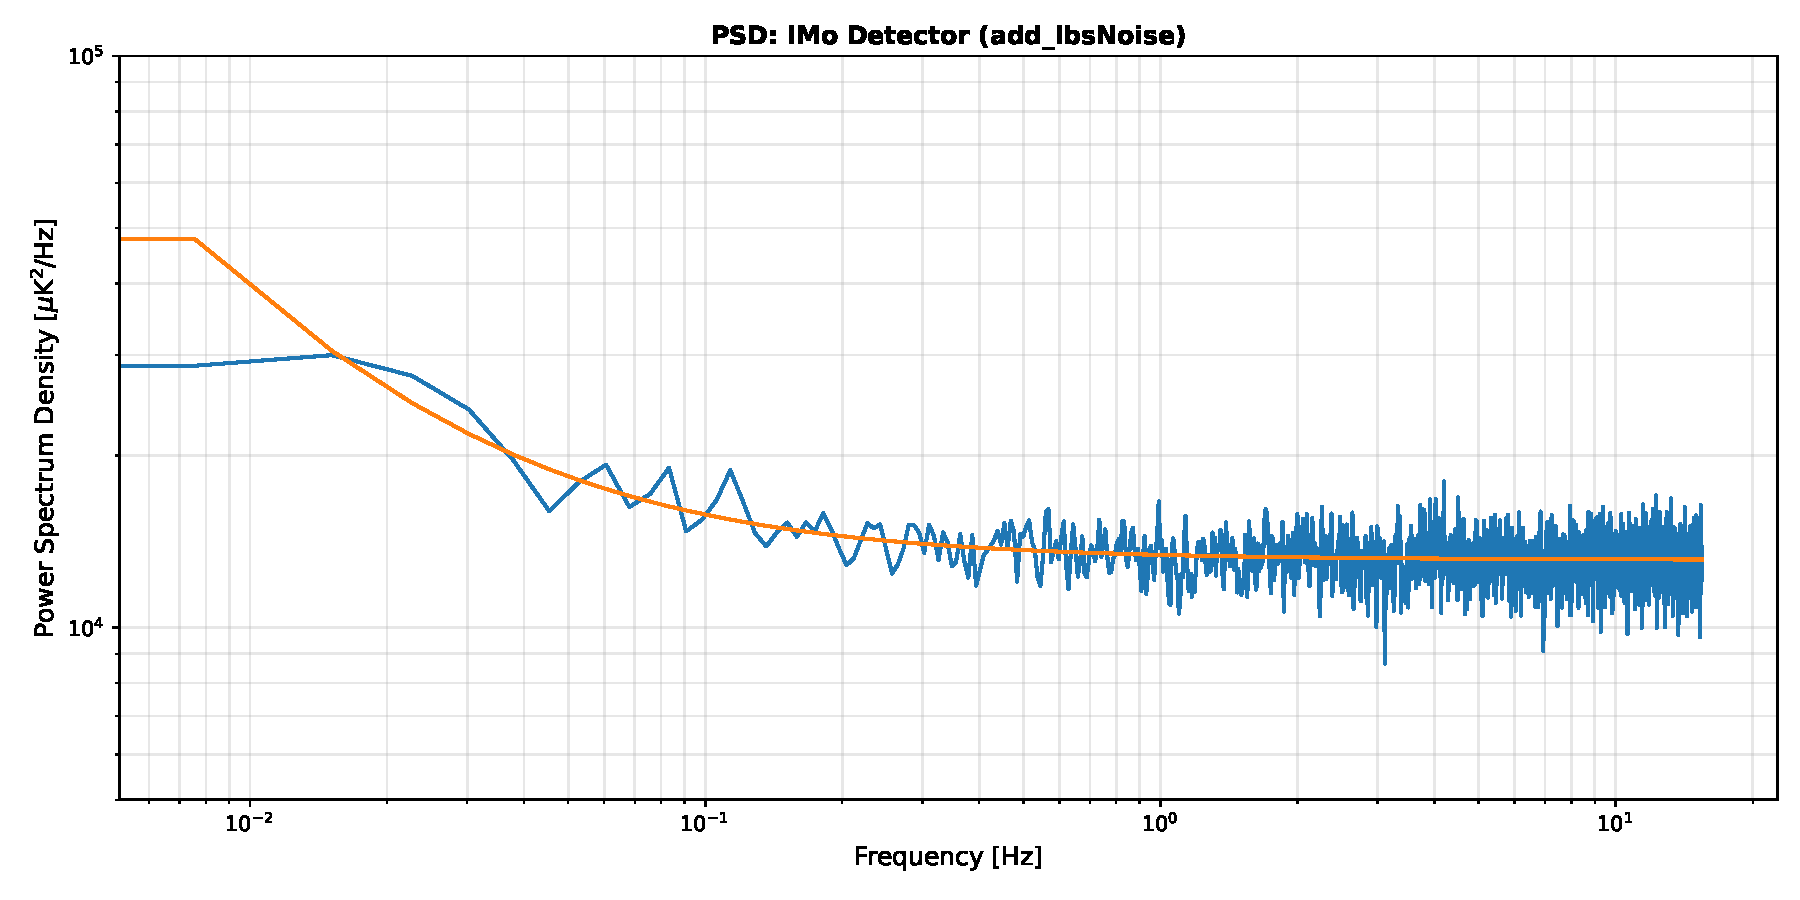
\includegraphics[width=0.68\textwidth]{psd_imo_lbs.pdf}
    \caption{PSD of the TOD simulated with the IMo detector using \texttt{add\_lbsNoise}.}
    \label{fig:psd_imo_lbs}
\end{figure}

\begin{figure}[h!]
    \centering
    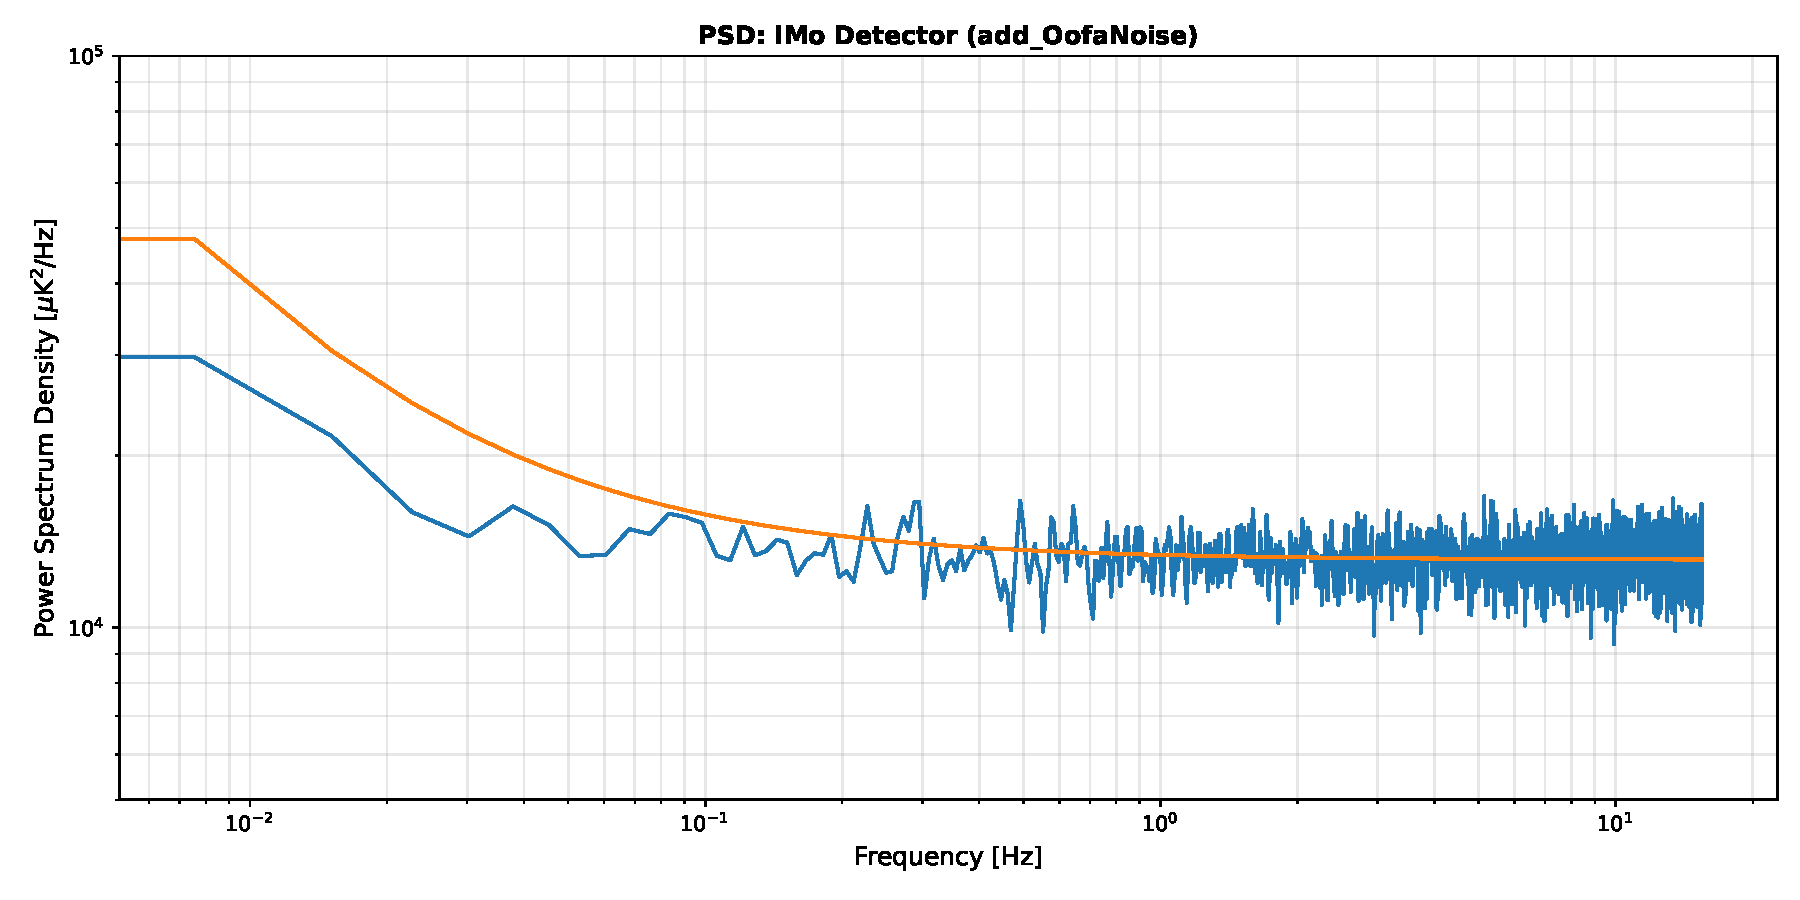
\includegraphics[width=0.68\textwidth]{psd_imo_oofa.pdf}
    \caption{PSD of the TOD simulated with the IMo detector using \texttt{add\_OofaNoise}.}
    \label{fig:psd_imo_oofa}
\end{figure}

These results confirm that both \texttt{add\_lbsNoise} and \texttt{add\_OofaNoise} correctly reproduce the target PSD for both detectors.

Although the comparison in the time and frequency domains provides an initial validation of the noise models, their real impact on cosmological observables only emerges at the map level. For this reason, in the next chapter the analysis is extended to long-duration simulations and to the construction of HEALPix maps.







